\section{Theorie}
\label{sec:Theorie}

Steckt ein Signal in einem Hintergrundrauschen, ist es nur erschwert möglich, 
dieses zu messen. Der Lock-In-Verstärker stellt eine Lösung für dieses Problem 
dar, indem das eingehende Rauschsignal $U_{sig}$ mit der Frequenz $\omega_0$ 
durch einen Bandpassfilter von hohen ($\omega \gg \omega_0$) und tiefen 
($\omega \ll \omega_0$) gelöst wird. Der Aufbau beinhaltet zusätzlich noch 
den Phasenschieber, dessen Aufgabe es ist, die Phasenlage des Referenzsignals 
so anzupassen, dass es synchron mit dem gemessenen Signal ist (Das ist nötig,
da die Ausgangsspannug $U_{out}$ von der Phasendifferenz zwischen Signal und 
Referenz abhängt). Am wichtigsten ist der Mischer, welcher zwischen alle 
Bestandteile geschlossen ist. An diesem werden die Signale $U_{sig}$ und $U_{ref}$
multipliziert. Letztlich dient der Tiefpassfilter als Glättung. Da das Produkt 
aus Signal und Referenz noch über Oberwellen verfügt, integriert dieser Filter 
(mit $\tau \gg \frac{1}{\omega_0}$) das Mischsignal $U_{sig} \texttimes U_{ref}$, 
was zur gewünschten Filterung der Rauschanteile führt. Somit wird am Ausgang 
eine Spannung gemessen für die gilt:
\begin{align}
    U_{out} \propto U_0 cos \varphi
\end{align}
Der Vorteil dieser Konstruktion liegt in der Güte, welche einen Wert von 
$Q = 100000$ erreichen kann. Wird die Zeitkonstante $\tau = RC$ sehr groß 
gewählt, so kann die Bandbreite $\increment \nu = \frac{1}{\pi RC}$ sehr klein 
gemacht werden. Ein einzelner Bandpass hingegen würde nur einen Bruchteil der 
Güte des Verstärkers erreichen. 

Es wird nun der Signalverlauf einer Sinusspannung $U_{sig} = U_0 sin (\omega t)$
betrachtet, welche durch einen auf eins normierte Rechteckspannung moduliert 
wird. Jenes ist in \autoref{fig:f1} dargestellt.
\begin{figure}[H]
    \centering
        \centering
        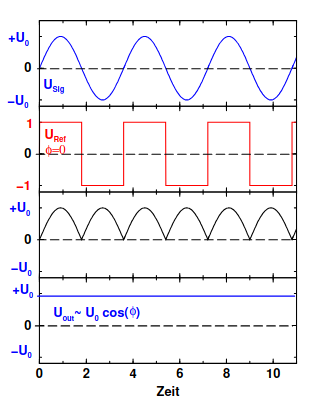
\includegraphics[width=0.45\textwidth]{Bilder/sigs.png}
        \caption{Signalverläufe. \cite{anleitung2}}
    \hfill
    \label{fig:f1}
\end{figure}
\noindent Die Rechteckspannung wird durch eine Fourierreihe approximiert, welche
sich aus der Grundfrequenz zusammensetzt.
\begin{equation}
    U_{ref} = \frac{4}{pi} \left(sin(\omega t) + \frac{1}{3}sin(3 \, \omega t) + \frac{1}{5}sin(5 \, \omega t) + ...\right)
\end{equation}
Der erste Term repräsentiert die Grundfrequenz, während die restlichen Terme 
die ungeraden harmonischen Vielfache sind. Das bereits erwähnte Produkt aus 
Signal- und Modulationsfrequenz nimmt folglich die Form
\begin{equation}
    U_{sig} \texttimes U_{ref} = \frac{2}{\pi} U_0 \left(1- \frac{2}{3}cos(2 \, \omega t) - \frac{2}{15}cos(4 \, \omega t) - \frac{2}{35}cos(6 \, \omega t) - ...\right)
\end{equation}
an. Nun wird der Tiefpassfilter relevant, dieser sorgt dafür, dass die Oberwellen 
entfernt werden. Die Ausgangsspannung ergibt sich demnach (unter Einbeziehung 
möglicher Phasendifferenzen) zu dem Term
\begin{equation}
    \label{eqn:4}
    U_{out} = \frac{2}{\pi} U_0 cos(\varphi).
\end{equation}
Bei gleicher Phase von $U_{sig}$ und $U_{ref}$, was bei $\varphi = 0$ der Fall
ist, entfällt der Cosinus-Term. Die Ausgangsspannung ist demnach wieder eine 
Signalspannung, welche proportional zur Gleichspannung ist.


\subsection{Fehlerrechnung}
Die gemessenen Werte unterliegen Messunsicherheiten und werden demnach im
Folgenden nicht als fehlerfrei angesehen. Die Fehler entstehen bei der
Bildung der Mittelwerte durch den Fehler des Mittelwerts und bei der
Regressionsrechnung sowie der Fehlerforpflanzung durch Python.
Der Fehler des Mittelwerts ist gegeben durch 
\begin{equation}
    \begin{aligned}
        \increment \overline{x} &= \sqrt{\overline{x^2\kern-0.1em} - \overline{x}^2} \\
                            &= \frac{\sqrt{\frac{1}{N-1} \sum\limits_{i=1}^N (x_i - \overline{x})^2}}{\sqrt{N}}.
    \end{aligned}
\end{equation}

Um Fehler einzubeziehen, wird die Gauß'sche Fehlerfortpflanzung verwendet:
\begin{equation}
    \label{eqn:8}
    \increment f = \sqrt{\left(\frac{\partial f}{\partial x}\right)^2 \cdot \left(\increment x\right)^2 + \left(\frac{\partial f}{\partial y}\right)^2 \cdot \left(\increment y\right)^2 + .... + \left(\frac{\partial f}{\partial z}\right)^2 \cdot \left(\increment z\right)^2}
\end{equation}